\pagestyle{myFancy}
\chapter{Yang-Mills Theories on the Lattice}
\section{The Yang-Mills Continuum Action}
The aim of this chapter is to discretize the Yang-Mills action on a hypercubic lattice in $4$ dimensions. In order to do so, the action is obtained firstly in the continuum, beginning from the simplest case, Quantum Electrodynamics.\\
This first section is based on material that can be found in standard textbooks on quantum field theory \cite{srednicki2007quantum, peskin1995introduction, weinberg1995quantum, kaku1993quantum, ramond1997field}, personal notes and computations.

\subsection{Scalar Fields}
In quantum field theory, a real scalar massive field is described, in a $4$-dimensional spacetime with metric $\eta_{\mu\nu} = \diag(-1,1,1,1)$, by the following Lorentz-covariant action (in natural units, where $c = \hslash = 1$):
\begin{equation}
    S[\phi] = \dV \pr{-\frac12 \partial^\mu\phi\partial_\mu\phi -\frac12 m^2\phi^2 +V(\phi)} \label{1:ActionScalar}
\end{equation}
where $V(\phi)$ is any potential, such as $\frac{g}{6}\phi^3$ or $\frac{g}{4!}\phi^4$.
Real scalar fields do not describe any real-world elementary particle, though they are useful to learn basic principles of quantum field theory, as they are the simplest fields that can be written.
%TODO: check notation consistency with lattice action after Wick rotation

\subsection{Dirac Spinor Fields}
Let us now take into consideration a (free) quantum field theory describing a fermion, such as a quark or a lepton. Its action can be written as:
\begin{equation}
      S_\psi[\psi(x),\psibar(x)] = \dV \left( \i\psibar\slashed\partial\psi - m\psibar\psi \right) \label{1:FreeQEDFermionAction}
\end{equation}
from which, upon the application of the variational principle, the Dirac equation follows:
\begin{equation}
    \left( \i\slashed\partial-m \right) \psi(x) = 0 \label{1:DiracEq}
\end{equation}
It can now be easily checked by direct computation that this action is invariant under a rigid (global) phase transformation, also called a global $U(1)$ transformation:
\begin{align*}
    \psi(x) &\rightarrow \psi'(x) = e^{-\i\alpha}\psi(x) \numthis\label{1:PhaseTransform} \\
    \psibar(x) &\rightarrow \psibar'(x) = \psibar(x) e^{\i\alpha}
\end{align*}
where $\alpha$ is a constant that does not depend on the spacetime coordinate $x$, because if $\alpha$ was a function of $x$, the kinetic term of the action \eqref{1:FreeQEDFermionAction} would not be invariant under such transformation.

\subsection{Quantum Electrodynamics\label{Sec:QED}}
As the free field theory itself is non interacting, it does not provide any real-world prediction, so it is useful to write an interacting action where the spinor field is coupled, for instance, to a vector field $A_\mu$, \ie the photon.
One way to implement this interaction is to ask for local, instead of global, invariance of the action \eqref{1:FreeQEDFermionAction} under the phase transformation \eqref{1:PhaseTransform}, where now $\alpha=\alpha(x)$.
In order to do so, the covariant derivative has to be defined as follows:
\begin{equation}
    D_\mu \equiv \partial_\mu+\i g A_\mu \label{1:QEDCovDeriv}
\end{equation}
where $g$ is the couplig constant.\footnote{Usually, in QED, $g$ is called $e$, the electron charge, though $g$ will be used in analogy to nonabelian gauge theories.}\\
The vector field's kinetic term is written in terms of its field-strength, namely:
\begin{align*}
    \Fmunu\equiv& -\frac{\i}{g}\left[D_\mu,D_\nu\right] = \\
    =& -\frac{\i}{g}\pr{D_\mu\pr{\partial_\nu+\i g A_\nu} - D_\nu\pr{\partial_\mu+\i g A_\mu}}=\\
    =& -\frac{\i}{g}\pr{\cancel{\partial_\mu\partial_\nu} + \i g\partial_\mu A_\nu -g^2A_\mu A_\nu - \cancel{\partial_\nu\partial_\mu} - \i g\partial_\nu A_\mu + g^2A_\nu A_\mu}=\\
    =& \partial_\mu A_\nu - \partial_\nu A_\mu + \i g\comm{A_\mu}{A_\nu}=\\
    =& \partial_\mu A_\nu - \partial_\nu A_\mu \numthis\label{1:FieldStrU1}
\end{align*}
where $\comm{A_\mu}{A_\nu}=A_\mu A_\nu-A_\nu A_\mu=0$ in the abelian theory.\\
Two different fields $A_\mu$ and $A_\mu'$ describe the same physics if one can be obtained from another through a gauge transformation:
\begin{align*}
    A_\mu'(x) =& A_\mu(x) + \frac1g \partial_\mu\alpha(x) \numthis\label{1:QEDGaugeTransf} \\
    \Fmunu' = \Fmunu + \frac1g&\left( \partial_\mu\partial_\nu-\partial_\nu\partial_\mu \right)\alpha(x) = \Fmunu
\end{align*}
Thus, the free action for the vector field is:
\begin{equation}
    S_{EM} = -\frac14\dV F_{\mu\nu}F^{\mu\nu} \label{1:FreeMaxwellAction}
\end{equation}
That is also gauge invariant, i.e. invariant under \eqref{1:QEDGaugeTransf}, as $\Fmunu$ is gauge invariant.\\
The term that broke the local phase invariance of the action \eqref{1:FreeQEDFermionAction} can now be ``absorbed'' by $A_\mu$ through a gauge transformation \eqref{1:QEDGaugeTransf}, thus making the full action gauge invariant:
\begin{align*}
    S_{QED} =& \dV\pr{\i\psibar\slashed{D}\psi-m\psibar\psi -\frac14\Fmunu F^{\mu\nu}} = \numthis\label{1:QEDaction}\\
    =& \dV\pr{\i\psibar\slashed{\partial}\psi-m\psibar\psi- g \psibar\slashed{A}\psi - \frac14\Fmunu F^{\mu\nu}}\\
    S_{QED} \rightarrow S_{QED}' =& \dV\pr{\i\psibar\slashed{\partial}\psi +\cancel{\psibar\slashed{\partial}\alpha\psi} -m\psibar\psi -g \psibar\slashed{A}\psi -\cancel{\psibar\slashed\partial\alpha\psi} -\frac14\Fmunu F^{\mu\nu}}=\\
    =& \dV\pr{\i\psibar\slashed{\partial}\psi-m\psibar\psi- g \psibar\slashed{A}\psi - \frac14\Fmunu F^{\mu\nu}} = S_{QED}
\end{align*}

\subsection{Non-Abelian Gauge Theories\label{Sec:NonAbelianGaugeTheories}}
Let us now consider a theory with $N$ fermions, all with the same mass $m$, described by the spinorial fields $\psi_i(x)$ with $i=1, \dots, N$.
These $N$ fermions represent the $N$ possible charges of the same particle\footnote{For example, if $N=3$ the $3$ possible charges are the color charges of QCD, as will be shown later.} and are not to be confused with, for instance, the different possible flavors of the quarks, that describe different particles with different masses.\\
Its free action is:
\begin{equation}
    S_\psi[\psi_i(x),\psibar_i(x)] = \sum_{i=1}^N\dV\pr{\i\psibar_i\slashed\partial\psi_i - m\psibar_i\psi_i} \label{1:FreeFermionAction}
\end{equation}
From now on, the sum over $i$ (and all other repeated latin indexes) will be omitted, unless differently specified.
This action is invariant under the global transformation:
\begin{align*}
    \psi_i(x) &\rightarrow \psi_i'(x) = \U\psi_j(x) \numthis\label{1:UNTransform}\\
    \psibar_i(x) &\rightarrow \psibar_i'(x) = \psibar_j(x)\Udag
\end{align*}
if $U$ is any (constant) $N\times N$ matrix such that $UU^\dagger = U^\dagger U = \id \Leftrightarrow U^\dagger=U^{-1}$, or in other words, if $U\in\UN$.
For this reason, this transformation is also called a global $\UN$ transformation.
The phase transformation \eqref{1:PhaseTransform} is the particular case where $U=e^{-\i\alpha}\in\Uem$, that is the only Abelian (commutative) unitary group.\\
As $\UN = \SUN\otimes\Uem$ $\forall N>1$, $U\in\SUN$ instead of $U\in\UN$ can be imposed, and will be from now on, without loss of generality.\\
In an analogous way to what has been done in\secref{Sec:QED}, this invariance can be made local by implementing a proper covariant derivative, similar to \eqref{1:QEDCovDeriv}.
In order to do so, the infinitesimal $\SUN$ transformation has to be considered:
\begin{equation}
    U_{ij}(x) = \delta_{ij} + \i\theta^a(x)\pr{T^a}_{ij} + O(\theta^2) \label{1:InfinitesimalSUN}
\end{equation}
where the indices $i$ and $j$ run from $1$ to $N$ (as before) and the index $a$ runs from $1$ to $N^2-1$ (the dimension of the group $\SUN$).
The matrixes $T^a$ are the $N^2-1$ generators of $\sun$ (the Lie algebra of $\SUN$), thus they are $\NxN$ hermitean and traceless, which obey the commutation relations:
\begin{equation}
    \comm{T^a}{T^b} = \i f^{abc}T^c \label{1:StrConstSUN}
\end{equation}
where $f^{abc}$ are called \emph{structure constants} of $\sun$. The normalization of these matrices can be chosen such that they obey the condition:
\begin{equation}
    \Tr(T^aT^b) = \frac12\delta^{ab} \label{1:NormCondSUN}
\end{equation}
some examples are:
\begin{itemize}
    \item $N=2$, $T^a=\frac{\sigma^a}{2}$, with $\sigma^a$ the Pauli matrices and $f^{abc}=\varepsilon^{abc}$;
    \item $N=3$, $T^a=\frac{\lambda^a}{2}$, with $\lambda^a$ the Gell-Mann matrices.
\end{itemize}
where $\varepsilon^{abc}$ is the completely antisymmetric Levi-Civita symbol.\\
The covariant derivative, therefore, is written as:
\begin{equation}
    D_\mu \equiv \partial_\mu + \i g \A_\mu(x) \label{1:CovDeriv}
\end{equation}
where an $N\times N$ identity matrix $\id$ multiplying $\partial_\mu$ has to be understood, and $\A_\mu(x)$ is a gauge field of $\SUN$, \ie a traceless, hermitean $N\times N$ matrix, or, in other words, $\A_\mu(x)\in\sun$.\\
The covariant derivative can be written more explicitly acting on the set of spinors $\psi_i$:
\begin{equation*}
    \pr{D_\mu}_{ij}\psi_j = \partial_\mu \id_{ij}\psi_j + \i g \pr{\A_\mu(x)}_{ij}\psi_j
\end{equation*}
In order for the action to be gauge invariant, the field $\A_\mu$ must satisfy the gauge transformation property
\begin{equation}
    \A_\mu(x) \rightarrow \A_\mu'(x) = U(x)\A_\mu(x)U^\dagger(x) - \frac{\i}{g}U(x)\partial_\mu U^\dagger(x) \label{1:GaugeTransformSUN}
\end{equation}
This expression is a little more complicated than \eqref{1:QEDGaugeTransf}, due to the fact that $\A_\mu$ is now a non-commuting matrix. However if the Abelian case $\Uem$ is taken into consideration, where $U(x)=e^{-\i\alpha(x)}$, \eqref{1:QEDGaugeTransf} follows directly from \eqref{1:GaugeTransformSUN}.\\
Now, it can be easily checked that the kinetic term of the Lagrangian
\begin{equation*}
    \Lagr_K = \i\psibar_i\slashed{D}\psi_i = \i\psibar_i\slashed\partial\psi_i -g\psibar_i\slashed\A\psi_i
\end{equation*}
is gauge invariant (\ie invariant under \eqref{1:UNTransform} and \eqref{1:GaugeTransformSUN}) through direct computation:
\begin{align*}
    \Lagr_K \rightarrow \Lagr_K' =& \i\psibar_i U^\dagger\slashed\partial\pr{U\psi_i} -g\psibar_i\underbrace{U^\dagger U}_{\id}\slashed\A\underbrace{U^\dagger U}_{\id}\psi_i +\i\psibar_i\underbrace{U^\dagger U}_{\id}\pr{\slashed\partial U^\dagger}U\psi_i= \\
    =& \i\psibar_i U^\dagger\pr{\slashed\partial U}\psi_i +\underbrace{\i\psibar_i\slashed\partial\psi_i -g\psibar_i\slashed\A\psi_i}_{\Lagr_K} +\i\psibar_i\pr{\slashed\partial U^\dagger}U\psi_i= \\
    =& \Lagr_K +\i\psibar_i\gamma^\mu\pr{U^\dagger\partial_\mu U+ \partial_\mu U^\dagger U}\psi_i= \\
    =& \Lagr_K +\i\psibar_i\gamma^\mu\partial_\mu\pr{U^\dagger U}\psi_i= \\
    =& \Lagr_K +\i\psibar_i\gamma^\mu\underbrace{\partial_\mu\pr{\id}}_{=0}\psi_i = \Lagr_K
\end{align*}
Because of this fact, it is directly implied that the covariant derivative \eqref{1:CovDeriv} must transform, under a gauge transformation, in the adjoint representation:
\begin{equation}
    D_\mu \rightarrow D_\mu' = U D_\mu U^\dagger \label{1:GaugeTrCovDer}
\end{equation}
The field-strength for the field $\A_\mu$ is obtained, as for the Abelian case, through the commutator of two covariant derivatives. The computation is the same as \eqref{1:FieldStrU1}, but this time the commutator term is non-vanishing:
\begin{equation}
    \Fmunu\equiv -\frac{\i}{g}\comm{D_\mu}{D_\nu} = \partial_\mu\A_\nu -\partial_\nu\A_\mu +\i g\comm{\A_\mu}{\A_\nu} \label{1:FieldStrDef}
\end{equation}
This expression can be simplified a little by considering that $\A_\mu$ and $\Fmunu$ are elements of $\sun$, thus writing them in terms of their components \wrt the basis $T^a$:
\begin{align}
    \A_\mu(x) =& A_\mu^a(x) T^a \label{1:AmuComp}\\
    \Fmunu(x) =& \Fmunu^a(x) T^a \label{1:FmunuComp}
\end{align}
and by considering the relation \eqref{1:StrConstSUN}:
\begin{align*}
    \Fmunu^aT^a =& \pr{\partial_\mu A_\nu^a-\partial_\nu A_\mu^a}T^a +\i g\comm{A_\mu^bT^b}{A_\nu^cT^c}= \\
    =& \pr{\partial_\mu A_\nu^a-\partial_\nu A_\mu^a}T^a +\i gA_\mu^bA_\nu^c\underbrace{\comm{T^b}{T^c}}_{if^{bca}T^a}= \\
    =& \pr{\partial_\mu A_\nu^a-\partial_\nu A_\mu^a -gf^{abc}A_\mu^bA_\nu^c}T^a \\
    \Fmunu^a =& \partial_\mu A_\nu^a-\partial_\nu A_\mu^a -gf^{abc}A_\mu^bA_\nu^c \numthis\label{1:FmunuExplComp}
\end{align*}
In order to write a kinetic action for the field $\A_\mu$, a term proportional to $\Fmunu F^{\mu\nu}$, like in \eqref{1:FreeMaxwellAction}, is not enough:
because of \eqref{1:GaugeTrCovDer} and the definition \eqref{1:FieldStrDef}, it must transform as $\Fmunu F^{\mu\nu}\rightarrow U\Fmunu F^{\mu\nu} U^\dagger$, therefore it would not be gauge invariant.
In fact a gauge invariant action, called Yang-Mills action, is:
\begin{equation}
    S_{YM} = -\frac12\dV\Tr\pr{\Fmunu F^{\mu\nu}} \label{1:YMAction}
\end{equation}
because of the ciclic property of the trace.\footnote{Actually, a term proportional to $\det\pr{\Fmunu^a F^{a\mu\nu}}$ would be gauge invariant as well, but it would not be a suitable kinetic term as it would involve terms of higher order than $2$ in the components $\Fmunu^a$}
This action can be written in components, using \eqref{1:FmunuComp} and the trace property \eqref{1:NormCondSUN}:
\begin{equation}
    S_{YM} = -\frac12\dV\Tr\pr{\Fmunu^a F^{b\mu\nu}T^aT^b} = -\frac14\dV\Fmunu^a F^{a\mu\nu} \label{1:YMActionComp}
\end{equation}
Here, there are two remarks that need to be done.
The first one is that, if the gauge group is taken to be $\Uem$, the action \eqref{1:YMActionComp} reduces to \eqref{1:FreeMaxwellAction}, as $a=1$ because the group $\Uem$ has only $1$ generator.
The second one is that, if non-Abelian gauge groups are taken into consideration, this action naturally introduces self-interacting cubic and quartic terms, because the structure constants $f^{abc}$ are non-vanishing. This is, for example, the case for the group $\SU(3)$, that is used to describe gluon interaction, \ie Quantum Chromodynamics (QCD).
These self-interactions make the the Yang-Mills action interesting to be studied even alone, without any other fermionic or bosonic interacting field, as it will be shown later.
\begin{comment}
\\Everything that has been said for $\SUN$ can be also extended to $\mathit{SO}(N)$ by replacing \emph{unitary} with \emph{orthogonal} and \emph{traceless} with \emph{antisymmetric}. In fact, this discussion can be made for every compact\footnote{Compactness, \ie $\Tr{T^aT^b}$ positive defined, is required in order to have a bounded from below Hamiltonian.} group, such as the symplectic group $\mathit{Sp}(2N)$ and the five exceptional Lie groups $\mathit{G}(2)$, $\spF$, $\mathit{E}(6)$, $\mathit{E}(7)$ and $\mathit{E}(8)$.
\end{comment}

\subsection{Wick Rotation}
Up to now, actions were written in Minkowskian spacetime, where $\eta_{\mu\nu} = \diag(-1,1,1,1)$. In order to have a positive-defined metric $\eta_{\mu\nu} = \delta_{\mu\nu}$ a Wick rotation can be performed by re-defining the time coordinate to be $\tau = \i t = \i x^0$, as is rigorously proven in \cite{SCHLINGEMANN_1999}.
The principle behind Wick rotation is that the time coordinate is promoted to be a complex number and the integration (in the action) from $-\infty$ to $\infty$ is made to be from $-\i\infty$ to $\i\infty$ through a rotation of $\frac\pi2$ in the complex plane, assuming that correlators and other physical quantities do not present singularities in the first and third quadrant of the complex plane of $t$.
This rotation is not only a matter of convenience, as it is needed in perturbative QFT for the computation of (otherwise oscillating) functional integrals and because a Minkowskian lattice cannot be rigorously defined.\\
The relation between the Minkowski actions written before and the Euclidean actions is $S^M = \i S^E$, because $\dd^4x^E = \i \dd^4x^M$.\\
Thus, the Euclidean actions are\footnote{Note that they are not the same as their Minkowskian counterpart, as some redefinitions of the fields and the $\gamma$ matrices have been implicitly made, in order to have the respective theories non ill-defined.}:
\begin{align}
    S^E[\phi] =& \dV \pr{\frac12\partial^\mu\phi\partial_\mu\phi+\frac12m^2\phi^2+V(\phi)} \label{1:ScalarActionEuclidean}\\
    S^E_F =& \dV\psibar\pr{\gamma^\mu\pr{\partial_\mu+\i g \A_\mu} + m}\psi \label{1:FerionActionEuclidean}\\
    S^E_{YM} =& \frac14 \dV \Fmunu^a F^{a\mu\nu} \label{1:YMActionEuclidean}
\end{align}
where the superscript $E$, meaning that the action is written in the Euclidean spacetime, will be omitted from now on.

\section{Lattice Field Theory}
\subsection{Why Lattice Field Theory}
After the Wick rotation, quantum field theory can be studied perturbatively through the saddle-point evaluation of the path integral, where the partition function
\begin{equation*}
    Z = \int\DD\varphi e^{\i S^M[\varphi]} = \int\DD\varphi e^{-S^E[\varphi]}
\end{equation*}
has become non-oscillating.
This approach, however, works well only if the coupling constants are \emph{small enough} and does not allow to obtain non-perturbative results, \ie physical quantities that depend on essential singularities in the coupling constant, like glueballs for Yang-Mills theories.\\
For this reason, a non-perturbative approach has to be taken into consideration and one possibility is Lattice Field Theory: the spacetime is discretized to a lattice, with lattice spacing $a$, and the fields can assume different values only on the sites of the lattice.
More in detail, a scalar field lives on lattice sites, a vector field lives on links between sites and objects with $k$ indices live on $k$-simplexes.\\
If the limit $a\to0$ is taken, the theory must reproduce results obtained in the continuum, like the ones obtained in perturbation theory in the regime where it can be applied, however the presence of a discrete spacetime provides a natural cutoff for the momenta, allowing ultraviolet divergencies to be kept under control, although they need to be taken into consideration when approaching the continuum limit.\\
In this section, based on standard quantum field theory textbooks cited before and lattice field theory textbooks \cite{Montvay:1994cy, Gattringer:2010zz, DeGrand:2006zz}, the regularization of the previous quantum field theories on a Simple Hypercubic (SH) lattice is presented.
A more detailed description of the geometric properties of the figures mentioned below can be found in \cite{coxeter2012regular}.
\subsection{Lattice}
A lattice $\Lambda$ in $\R^D$ is defined as the set of all possible linear combinations with integer coefficients of the vectors $\prc{v_i}$, which form a basis of $\R^D$.
Formally:
\begin{equation}
    \Lambda =\left\{\left.\sum _{i=1}^{D}c_{i}v_{i}\;\right\vert \;c_{i}\in \mathbb {Z} \right\} \label{1:genericLattice}
\end{equation}

\subsubsection{Simple Hypercubic Lattice}
If the basis $\prc{v_i}$ is taken to be orthonormal, the lattice is called \emph{Simple Hypercubic}\footnote{The word \emph{simple} is used to make a distinction with the Body-Centered Hypercubic lattice, in the following sections.}.\\
In figure \eqref{1F:cubicLattice} is represented a portion of a Simple Hypercubic lattice in $D=3$.
\begin{figure}[h!]
    \centering
    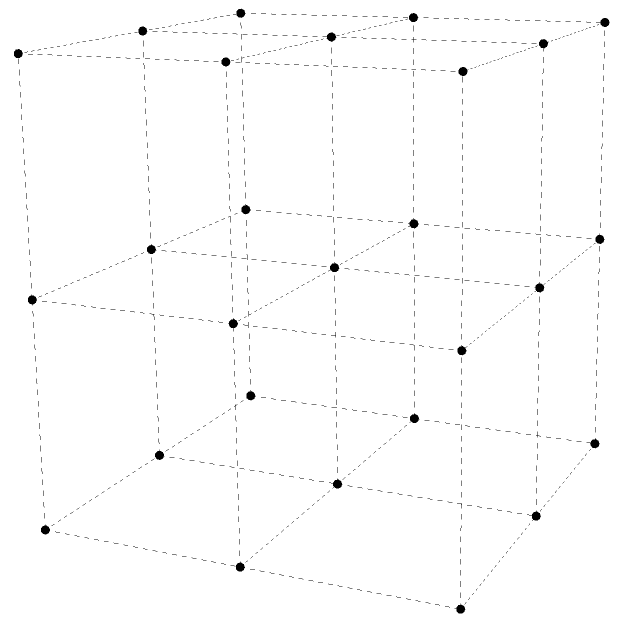
\includegraphics[width=0.25\textwidth]{Lattice.png}
    \caption{A cubic lattice.}
    \label{1F:cubicLattice}
\end{figure}\\
For the SH lattice in $D=4$, the fundamental region (the smallest $D$-dimensional polyhedron) is a $4$-dimensional hypercube, also called a tesseract.
This means that a SH lattice can be seen as a tassellation of the spacetime with tesseracts as elementary cells.
Each point of the lattice has $8$ nearest neighbours that are identified by the vectors obtained through all possible permutations of position and sign of $(\pm1,0,0,0)$.\\
The plaquette (the simplest bidimensional figure) is a square.
This will be important when implementing gauge theories on the lattice.

\subsubsection{Body-Centered Tesseract}
The SH lattice is not, of course, the only possible choice of a lattice in $4$ spacetime dimensions.
Another common choice, already used to simulate gauge theories~\cite{Celmaster:1982ht}, is the Body-Centered Tesseract (BCT).
It consists of packing the spacetime with tesseracts, as the name suggests, but considering both the corners and the centers of every hypercube as lattice sites.
Every site has, therefore, $24$ nearest neighbours: $16$ are identified by all possible permutations of signs of $\pr{\pm\frac12,\pm\frac12,\pm\frac12,\pm\frac12}$, the $8$ remaining are the ones of the SH lattice.\\
The cell of this lattice is known as $24$-cell and the plaquettes are triangular.

\subsection{Scalar Fields on the Simple Hypercubic Lattice}
Let us consider a simple hypercubic lattice $\Lambda_{SH}$ extending over $L=L_1=L_2=L_3$ lattice spacings in the spatial directions and over $T=L_0$ lattice spacings in the temporal direction.
Let us also consider a scalar field $\phi(x)$ in order to introduce some useful tools that will be needed later.
As anticipated at the beginning of this section, a scalar field can only assume values on the sites of the lattice, therefore $x\in\Lambda_{SH}$, and let us assume, for simplicity, periodic boundary conditions on the field, therefore $\phi(x+a\hat\mu L_\mu)=\phi(x)$.
The Fourier transform of the field becomes
\begin{equation}
    \tilde\phi(p)=\sum_x a^4 e^{-\i p\cdot x}\phi(x) \label{1:FourierScalar}
\end{equation}
and the allowed momenta are given by
\begin{equation}
    p_\mu=\frac{2\pi}{aL_\mu}n_\mu, \qquad n_\mu=0, \dots, L_3 \label{1:Brillouin}
\end{equation}
This ensures that the momenta can take only the assigned values of the Brillouin zone \eqref{1:Brillouin} and therefore cannot go to infinity, providing a natural cutoff given by the lattice spacing $a$.
The discretization also implies that derivatives of the fields cannot be computed, therefore the lattice forward derivative is used:
\begin{equation}
    \partial_\mu\phi(x)\rightarrow\frac{\phi(x+a\hat\mu)-\phi(x)}{a} \label{1:ForwardLatticeDerivative}
\end{equation}\\
Assuming a self-interaction potential $V(\phi)=\frac\lambda{4!}\phi^4$, the action \eqref{1:ActionScalar} can be written in terms of the lattice in the following way:
\begin{equation}
    S=a^4\sum_x\pr{\frac1{2a^2}\prs{\phi(x+a\hat\mu)-\phi(x)}^2+\frac12m^2\phi^2(x)+\frac\lambda{4!}\phi^4(x)} \label{1:ScalarActionLattice}
\end{equation}
A similar approach will be used in the following section to obtain the action for Yang-Mills theories.

\subsection{Gauge Fields on the Simple Hypercubic Lattice}
Let us now take into consideration a Yang-Mills theory, as in\secref{Sec:NonAbelianGaugeTheories}.
As anticipated before, gauge fields, being vector fields, can assume value only on links between sites of the lattice.
One could naively think that putting gauge vectors $A_\mu(x)$ on the links is enough, but this would explicitly break gauge invariance.
For this reason, Wilson's idea was to put the gauge group (and not algebra) elements, namely $U_\mu(x) = e^{\i g A_\mu(x)}$.\\
The field $U_\mu(x)$ lives on the link connecting the site $x$ with the site $x+a\hat\mu$, therefore the link is oriented and link variables in negative directions can also be defined:\\
$U_{-\mu}(x) \equiv U^\dagger_\mu(x-a\hat\mu)$.
\begin{figure}[h!]
    \includegraphics[width=\textwidth]{linkVariables.png}
    \caption{Schematic visualization of link variables.}
    \label{1F:LinkVariables}
\end{figure}\\
Under a gauge transformation, the fields $U_\mu$ transform according to the following relation:
\begin{equation}
    U_\mu(x)\rightarrow \Omega(x) U_\mu(x) \Omega^\dagger(x+a\hat\mu) \label{1:GaugeTransformLinkVariable}
\end{equation}
where $\Omega(x)$ is any $\SUN$ matrix at the point $x$ on the lattice.
As a consequence of this relation, the trace of any product of links forming a closed path is a gauge-invariant quantity, thanks to the cyclic property of the trace.\\
With this in mind, Wilson's idea was to choose the simplest closed path possible: the plaquette, that in the simple hypercubic lattice is a square.
The product of link variables along a plaquette is defined in the following way:
\begin{align*}
    U_{\mu\nu}(x) \equiv& U_\mu(x)U_\nu(x+\hat\mu)U_{-\mu}(x+\hat\mu+\hat\nu)U_{-\nu}(x+\hat\nu) =\\
    =& U_\mu(x)U_\nu(x+\hat\mu)U^\dagger_\mu(x+\hat\nu)U^\dagger_\nu(x) \numthis\label{1:Plaquette}
\end{align*}
%TODO: Set a=1
Thus a gauge-invariant action, called Wilson action, can be written as follows:
\begin{equation}
    S_W[U]=\frac\beta{2N}\sum_{x\in\Lambda}\sum_{\mu<\nu}\Re\Tr[\id-U_{\mu\nu}(x)] \label{1:WilsonAction}
\end{equation}
